%
% Chapter 9
%

\chapter{SIGNAL EXTRACTION}
Despite the event selection being aimed at selecting signal and rejecting background, the signal region yields are dominated by background events,
and lack sufficient statistics to identify the presence of the \tth signal in data. These post-selection (pre-fit) yields are in Table~\ref{tab:yields} below.
Becuse the post-selection yields offer no discernable way of separating the signal in the data, additional discrimination is necessary. A multivariate strategy
relying on Boosted Decision Trees (BDTs) is used to further discriminate the \tth signal from various backgrounds. 

\begin{table}[htbp]
\begin{center}
  \caption[Signal region event yields by lepton flavor]{Expected yields for signal and background processes, and observed yields in data (pre-fit). Uncertainties shown
are purely statistical.}
    \begin{tabular}{l c c c} \hline
& $\mu\mu$ & $ee$ & $e\mu$  \\ \hline 
$t\bar{t}W$ & 45.4 $\pm$ 0.5 & 17.8 $\pm$ 0.3 & 64.3 $\pm$ 0.6 \\
$t\bar{t}Z/\gamma^{*}$ & 16.8 $\pm$ 0.7 & 14.8 $\pm$ 0.8 & 41.7 $\pm$ 1.4 \\
%\hline
%Diboson & 7460 $\pm$ 1060 & 3190 $\pm$ 680 & 289 $\pm$ 83 \\
%Rare SM. bkg & 7460 $\pm$ 1060 & 3190 $\pm$ 680 & 289 $\pm$ 83 \\
%Conversions & - & 172 $\pm$ 93 & 149 $\pm$ 82 \\
\hline
Charge flip & - & 172 $\pm$ 93 & 149 $\pm$ 82 \\
Non-prompt leptons & 29.9 $\pm$ 1.2 & 17.3 $\pm$ 1.1 & 53.5 $\pm$ 1.8 \\
\hline
Total bkg & 107.3 $\pm$ 1.7 & 70.3 $\pm$ 1.8 & 208.0 $\pm$ 2.9 \\
 \hline
$t\bar{t}H$ & 18.5 $\pm$ 0.2 & 7.4 $\pm$ 0.1 & 26.2 $\pm$ 0.2 \\
 \hline
Data & 154 & 95 & 274 \\
\hline
\end{tabular}
    \label{tab:yields}
\end{center}
\end{table}

%% \begin{figure}[hbtp]
%%  \begin{center}
%%    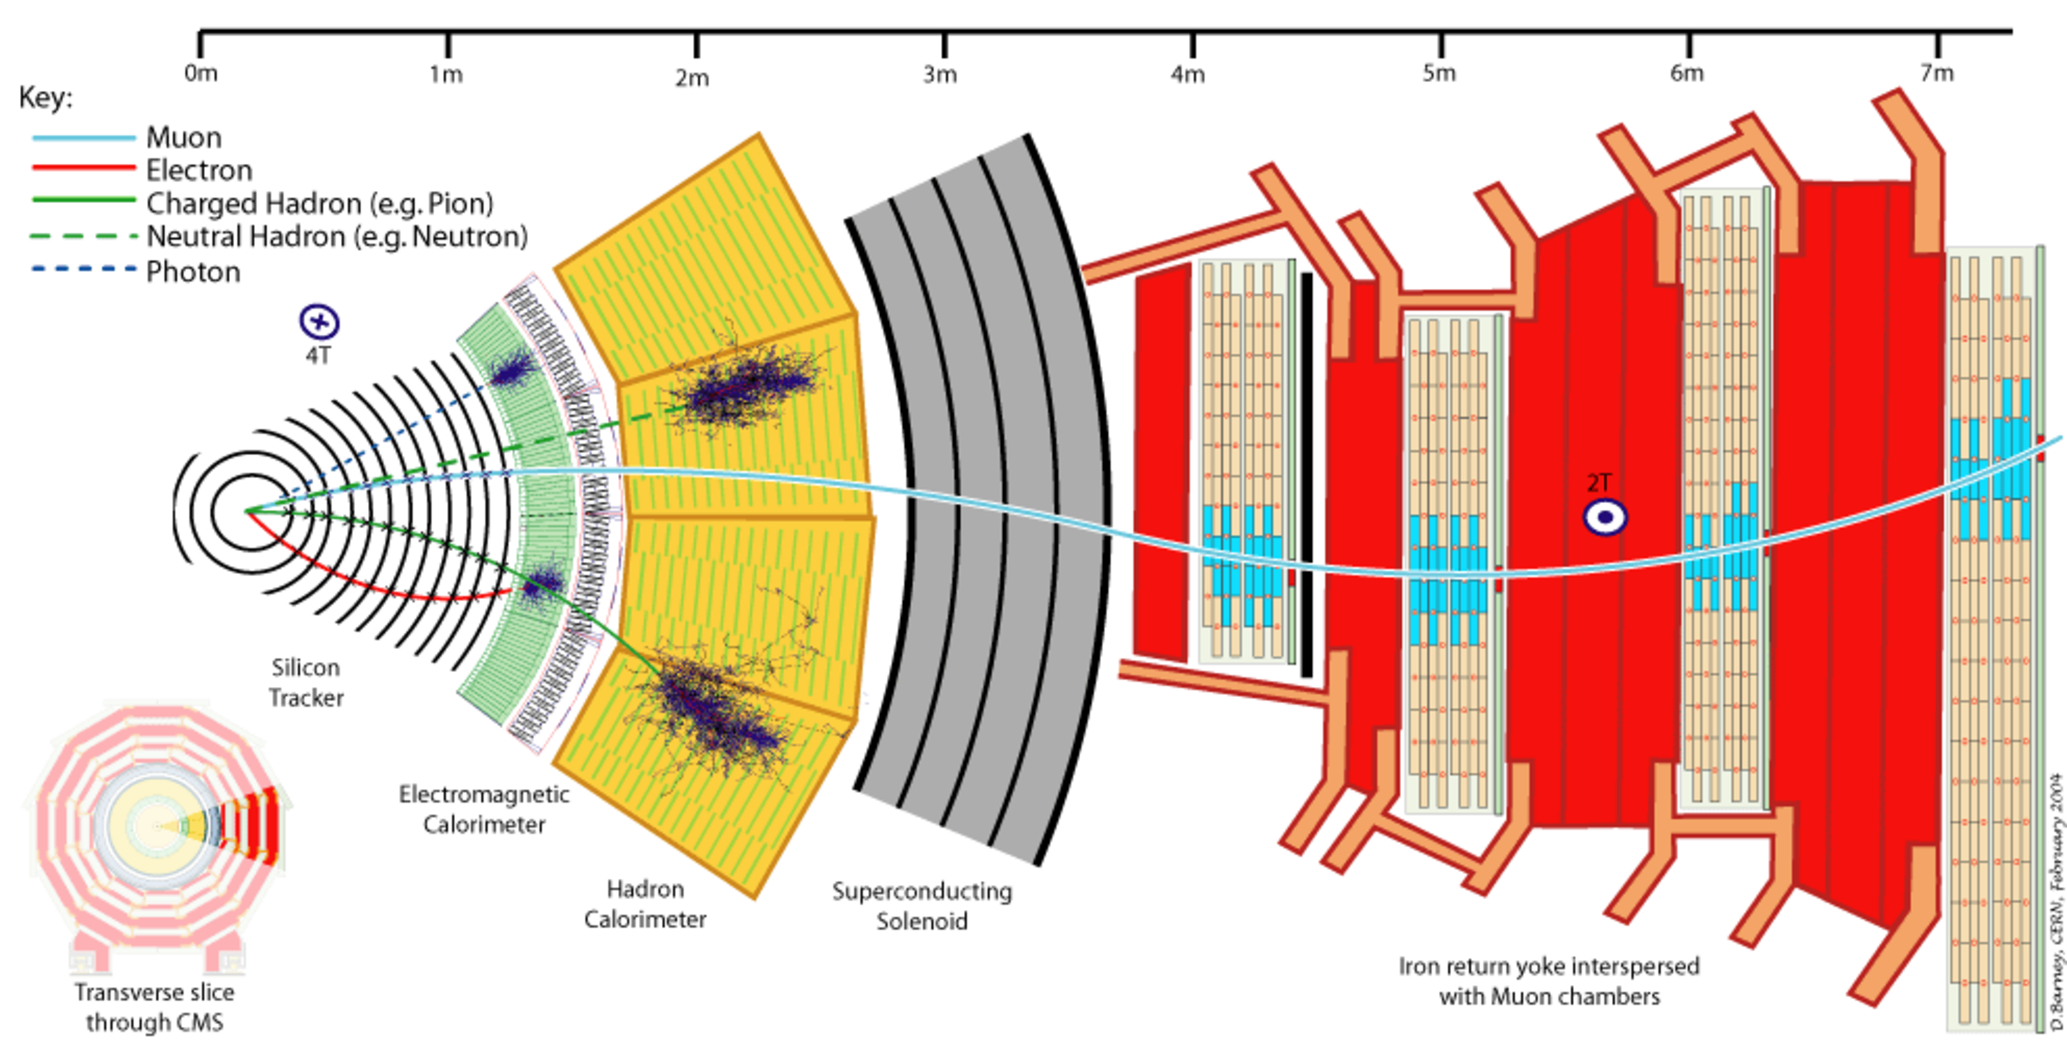
\includegraphics[width=0.8\textwidth]{ch4_figs/cms_particleflow.pdf}
%%    \caption{An overview of how CMS detects different types of particles. The slice of CMS in in the x-y plane.~\cite{NEED CITATION}.}
%%    \label{fig:cms_pflow}
%%  \end{center}
%% \end{figure}
